%============================================================================%
%
%	DOCUMENT DEFINITION
%
%============================================================================%

\documentclass[10pt,A4]{article}


%----------------------------------------------------------------------------------------
%	ENCODING
%----------------------------------------------------------------------------------------

%we use utf8 since we want to build from any machine
\usepackage[utf8]{inputenc}

%----------------------------------------------------------------------------------------
%	LOGIC
%----------------------------------------------------------------------------------------

% provides \isempty test
\usepackage{xifthen}

%----------------------------------------------------------------------------------------
%	FONT
%----------------------------------------------------------------------------------------

\usepackage[light,math]{iwona}

% set font default
\renewcommand*\familydefault{\sfdefault}
\usepackage[T1]{fontenc}

% more font size definitions
\usepackage{moresize}

\usepackage{fontawesome}

\usepackage{cancel}

%----------------------------------------------------------------------------------------
%	PAGE LAYOUT  DEFINITIONS
%----------------------------------------------------------------------------------------

%define page styles using geometry
\usepackage[a4paper]{geometry}

% for example, change the margins to 2 inches all round
\geometry{top=1cm, bottom=-.6cm, left=0.4cm, right=1cm}


%less space between header and content
\setlength{\headheight}{-5pt}

%indentation is zero
\setlength{\parindent}{0mm}

%----------------------------------------------------------------------------------------
%	TABLE /ARRAY DEFINITIONS
%----------------------------------------------------------------------------------------

%for layouting tables
\usepackage{multicol}
\usepackage{multirow}

%extended aligning of tabular cells
\usepackage{array}

\newcolumntype{x}[1]{%
>{\raggedleft\hspace{0pt}}p{#1}}%


%----------------------------------------------------------------------------------------
%	GRAPHICS DEFINITIONS
%----------------------------------------------------------------------------------------

%for header image
\usepackage{graphicx}

%for floating figures
\usepackage{wrapfig}
\usepackage{float}
%\floatstyle{boxed}
%\restylefloat{figure}

%for drawing graphics
\usepackage{tikz}
\usetikzlibrary{shapes, backgrounds,mindmap, trees}


%----------------------------------------------------------------------------------------
%	Color DEFINITIONS
%----------------------------------------------------------------------------------------
\usepackage{transparent}
\usepackage{color}

%accent color
\definecolor{complcol}{RGB}{250,150,10}

%dark background color
\definecolor{bgcol}{RGB}{110,110,110}

%light background / accent color
\definecolor{softcol}{RGB}{225,225,225}

\definecolor{sectcol}{RGB}{0,120,150}


%============================================================================%
%
%
%	DEFINITIONS
%
%
%============================================================================%

% returns minipage width minus two times \fboxsep
% to keep padding included in width calculations
\newcommand{\mpwidth}{\linewidth-\fboxsep-\fboxsep}


%----------------------------------------------------------------------------------------
% 	ARROW GRAPHICS in Tikz
%----------------------------------------------------------------------------------------

% a six pointed arrow poiting to the left
\newcommand{\tzlarrow}{(0,0) -- (0.2,0) -- (0.3,0.2) -- (0.2,0.4) -- (0,0.4) -- (0.1,0.2) -- cycle;}

% include the left arrow into a tikz picture
% param1: fill color
%
\newcommand{\larrow}[1]
{\begin{tikzpicture}[scale=0.58]
	 \filldraw[fill=#1!100,draw=#1!100!black]  \tzlarrow
 \end{tikzpicture}
}

% a six pointed arrow poiting to the right
\newcommand{\tzrarrow}{ (0,0.2) -- (0.1,0) -- (0.3,0) -- (0.2,0.2) -- (0.3,0.4) -- (0.1,0.4) -- cycle;}

% include the right arrow into a tikz picture
% param1: fill color
%
\newcommand{\rarrow}
{
\begin{tikzpicture}[scale=0.7]
	\filldraw[fill=sectcol!100,draw=sectcol!100!black] \tzrarrow
 \end{tikzpicture}
}

%----------------------------------------------------------------------------------------
%	custom sections
%----------------------------------------------------------------------------------------

% create a coloured box with arrow and title as cv section headline
% param 1: section title
%
\newcommand{\cvsection}[1]
{
\colorbox{sectcol}{\mystrut \makebox[1\mpwidth][l]{
\larrow{bgcol} \hspace{-8pt} \larrow{bgcol} \hspace{-8pt} \larrow{bgcol} \textbf{\textcolor{white}{\uppercase{#1}}}\hspace{4pt}
}}\\
}

% create a coloured arrow with title as cv meta section section
% param 1: meta section title
%
\newenvironment{metasection}[1] {
	\vspace{2pt}
	\begin{center}
		\textcolor{white}{\large{\uppercase{#1}}}\\
	\normalsize
	\parbox{0.7\mpwidth}{\textcolor{white}	\hrule}
}{\end{center}}

%----------------------------------------------------------------------------------------
%	 CV EVENT
%----------------------------------------------------------------------------------------

% creates a stretched box as cv entry headline followed by two paragraphs about
% the work you did
% param 1:	event time i.e. 2014 or 2011-2014 etc.
% param 2:	event name (what did you do?)
% param 3:	institution (where did you work / study)
% param 4:	what was your position
% param 5:	some words about your contributions
%
\newcommand{\cvevent}[5]
{
	\begin{tabular*}{1\mpwidth}{p{0.55\mpwidth}  x{0.42\mpwidth}}
 	\textcolor{black}{\textbf{#2}} & \textcolor{complcol}{#3}, \textcolor{bgcol}{#1}

	\end{tabular*}
% \textcolor{softcol}{\hrule}
% \vspace{6pt}
% 	\begin{tabular*}{0.5\mpwidth}{p{\mpwidth}}
% \larrow{softcol} #4\\[3pt] % (Add to the end of the line is an arrow: Ex: \larrow{softcol} #4\\[3pt])
% \larrow{softcol} #5\\[6pt]
% 	\end{tabular*}
}

% creates a stretched box as
\newcommand{\cveventmeta}[2]
{
	\mbox{\mystrut \hspace{87pt}\textit{#1}}\\
	#2
}

%----------------------------------------------------------------------------------------
% CUSTOM STRUT FOR EMPTY BOXES
%----------------------------------------- -----------------------------------------------
\newcommand{\mystrut}{\rule[-.3\baselineskip]{0pt}{\baselineskip}}

%----------------------------------------------------------------------------------------
% CUSTOM LOREM IPSUM
%----------------------------------------------------------------------------------------
\newcommand{\lorem}
{Lorem ipsum dolor sit amet, consectetur adipiscing elit. Donec a diam lectus.}


% use to vertically center content
% credits to: http://tex.stackexchange.com/questions/7219/how-to-vertically-center-two-images-next-to-each-other
\newcommand{\vcenteredinclude}[1]{\begingroup
\setbox0=\hbox{\includegraphics{#1}}%
\parbox{\wd0}{\box0}\endgroup}

% use to vertically center content
% credits to: http://tex.stackexchange.com/questions/7219/how-to-vertically-center-two-images-next-to-each-other
\newcommand*{\vcenteredhbox}[1]{\begingroup
\setbox0=\hbox{#1}\parbox{\wd0}{\box0}\endgroup}

%----------------------------------------------------------------------------------------
%	ICON-SET EMBEDDING
%----------------------------------------------------------------------------------------

% at this point we simplify our icon-embedding by simply referring to a set of png images.
% if you find a good way of including svg without conflicting with other packages you can
% replace this part
\newcommand{\icon}[3]{\makebox(#2, #2){\textcolor{#3}{\csname fa#1\endcsname}}}	%icon shortcut
\newcommand{\icontext}[4]{ 						%icon with text shortcut
	\vcenteredhbox{\icon{#1}{#2}{#4}} \vcenteredhbox{\textcolor{#4}{#3}}
}



%============================================================================%
%
%
%
%	DOCUMENT CONTENT
%
%
%
%============================================================================%
\begin{document}
\colorbox{white}{\begin{minipage}[c][0.95\textheight][t]{0.69\linewidth}


%---------------------------------------------------------------------------------------
%	TITLE HEADLINE
%----------------------------------------------------------------------------------------
\vspace{-3pt}
% use this for multiple words like working titles etc.
\colorbox{bgcol}{\makebox[0.985\linewidth][c]{\hspace{10pt}\HUGE{\textcolor{white}{\uppercase{Duc Anh Pham}} } \textcolor{sectcol}{\rule[-1mm]{1mm}{0.9cm}} \parbox[b]{5cm}{\large{ \textcolor{white}{{RECRUITING POSITION}}}\\
\large{ \textcolor{white}{{Software Development Intern}}}}
}}


%----------------------------------------------------------------------------------------
%	HEADER IMAGE
%----------------------------------------------------------------------------------------
\vspace{-6pt}
\begin{center}
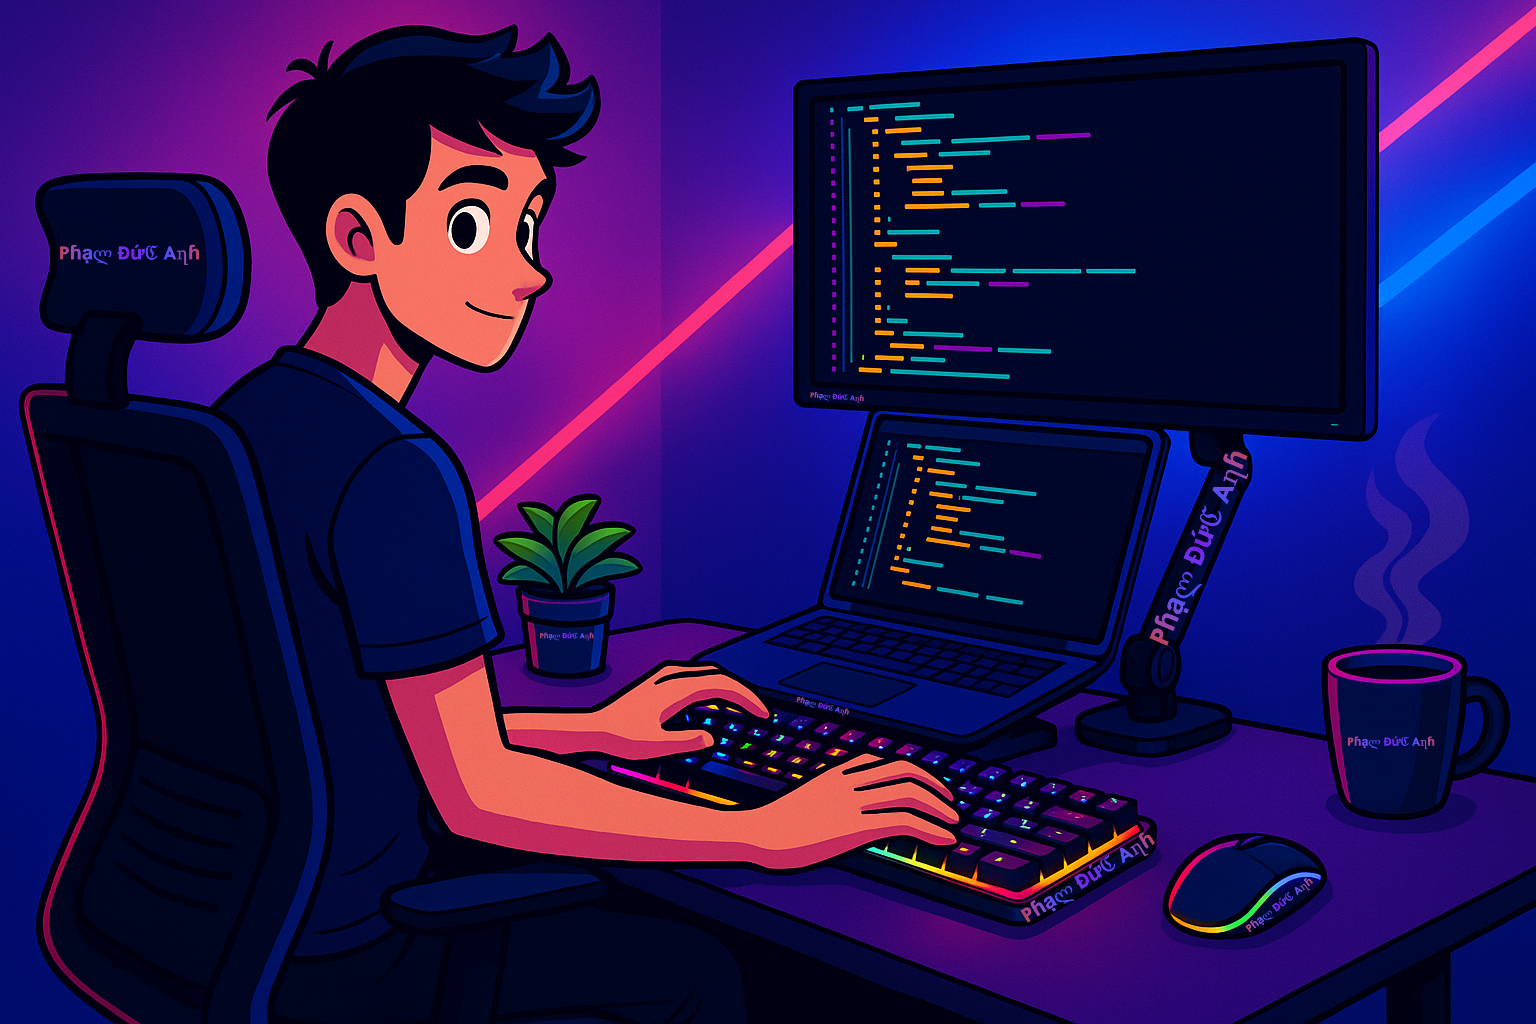
\includegraphics[height=3.5cm,width=13cm]{../img/avatar.png}
\end{center}
%---------------------------------------------------------------------------------------
%	SUMMARY
%----------------------------------------------------------------------------------------

\vspace{-3pt}

\cvsection{About Me}

\colorbox{bgcol}{
	\parbox{0.967\linewidth}{
		\begin{center}
		\larrow{sectcol}\larrow{sectcol}\textcolor{white}{I am a passionate Software Developer with experience in web application and software system development. Possess problem solving and teamwork skills, with a proactive approach to work. Eager to apply knowledge and learn from industry experts.}
		\end{center}
	}
}
\vspace{6pt}


%============================================================================%
%
%	CV SECTIONS AND EVENTS (MAIN CONTENT)
%
%============================================================================%

%---------------------------------------------------------------------------------------
%	SKILL
%----------------------------------------------------------------------------------------
\cvsection{Skill}
\vspace{-1.2em}

\begin{itemize}
	\item Basic English reading comprehension
    \item Attitude: Positive, proactive in work
    \item Working in groups: listening, coordinating
    \item Basic programming skills, eager to learn more
    \item Study hard and be willing to accept feedback from others
\end{itemize}

%---------------------------------------------------------------------------------------
%	EXPERIENCE
%----------------------------------------------------------------------------------------
\cvsection{Experience}

\cvevent{2021-2022}{NETWORKING GROUP LEADER}{University of Greenwich}{}{}
\vspace{-0.5em}

\begin{itemize}
    \item \textbf{August-2022}\\
	Design and build simulation configuration of network infrastructure system using Cisco Packet Tracer and Visio tools for a company preparing to go into operation.
\end{itemize}
\vspace{-0.5em}

\textcolor{bgcol}{\hrule}
\vspace{6pt}

\cvevent{2022-2023}{PROJECT DESIGN AND CONSTRUCTION}{University of Greenwich}{}{}
\vspace{-0.5em}

\begin{itemize}
    \item \textbf{September-2022} \textbf{SQL Server Design}\\
    Online library storage and management

    \item \textbf{November-2022} \textbf{Design and program the first Web project}\\
    Design and Build a website to sell phone cases using HTML, CSS, JS, jQuery, PHP, MySQL

    \item \textbf{March-2023} \textbf{Design and program the first e-commerce project}\\
	Design and build a website selling a full range of equipment, fruits and vegetables using ClickUp, HTML, CSS, JS, jQuery, PHP Laravel, MySQL, GitHub, Bootstrap. Apply MVC Model and Waterfall Software Development Lifecycle.
\end{itemize}
\vspace{-0.5em}

\textcolor{bgcol}{\hrule}
\vspace{6pt}

\cvevent{2024-2025}{FINAL PROJECT}{University of Greenwich}{}{}
\vspace{-0.5em}

\begin{itemize}
    \item \textbf{June 2025}\\
	Design and build a website to schedule an online medical exam with interesting functions using Jira, Figma, HTML, CSS, JS, jQuery, Thymeleaf, Java, PostgreSQL, GitHub, Bootstrap, Docker. Apply Restful API and Selected Methodology: Agile Software Development Lifecycle.
\end{itemize}

\vspace{3pt}

%---------------------------------------------------------------------------------------
%	EDUCATION SECTION
%--------------------------------------------------------------------------------------
\cvsection{Education}

\cvevent{Summer 2021- Summer 2025}{Bachelor Of Information Technology}{University of Greenwich}{}{}

\vspace{6px}

\cvsection{Achievement}

\cvevent{August 2023}{The best student of the subject: Security}{Greenwich International Bachelor Program}{}{}

\end{minipage}}%
\fcolorbox{white}{sectcol}{\begin{minipage}[c][0.95\textheight][t]{0.33\linewidth}


\begin{metasection}{Contact}

	\icontext{MapMarker}{12}{210/16A CMT8 St. Wd.10, Dist.3 HCMC}{white}\\[6pt]
	\icontext{MobilePhone}{12}{(+84)943206863}{white}\\[6pt]
	\icontext{EnvelopeO}{12}{ducanh040202003@gmail.com}{white}\\[6pt]
	\icontext{Github}{12}{github.com/ducanhphamorg}{white}\\[6pt]
	\icontext{Linkedin}{12}{linkedin.com/in/ducanhphamorg}{white}\\[6pt]
	\icontext{Facebook}{12}{facebook.com/ducanhphamorg}{white}\\[6pt]
\end{metasection}

%----------------------------------------------------------------------------------------
%	META SECTION
%----------------------------------------------------------------------------------------

\begin{metasection}{Fields}

\icontext{Code}{12}{Software Development}{white}\\
\icon{Star}{12}{complcol}\icon{Star}{12}{complcol}\icon{Star}{12}{complcol}\icon{Star}{12}{complcol}\icon{Star}{12}{complcol}\icon{Star}{12}{white}\icon{Star}{12}{white}\icon{Star}{12}{white}\icon{Star}{12}{white}\icon{Star}{12}{white}\\[6pt]

\icontext{CommentsO}{12}{Consulting}{white}\\
\icon{Star}{12}{complcol}\icon{Star}{12}{complcol}\icon{Star}{12}{complcol}\icon{Star}{12}{complcol}\icon{Star}{12}{complcol}\icon{Star}{12}{complcol}\icon{Star}{12}{complcol}\icon{Star}{12}{white}\icon{Star}{12}{white}\icon{Star}{12}{white}\\[6pt]

\icontext{CodeFork}{12}{Project Management}{white}\\
\icon{Star}{12}{complcol}\icon{Star}{12}{complcol}\icon{Star}{12}{complcol}\icon{Star}{12}{complcol}\icon{Star}{12}{white}\icon{Star}{12}{white}\icon{Star}{12}{white}\icon{Star}{12}{white}\icon{Star}{12}{white}\icon{Star}{12}{white}\\[6pt]


\end{metasection}


\begin{metasection}{BASIC TECHNOLOGIES}

\textcolor{white}{
\icontext{Code}{12}{HTML, CSS, Bootstrap}{white} \\[6pt]
\icontext{Code}{12}{JavaScript, jQuery}{white} \\[6pt]
\icontext{Code}{12}{Java, Thymeleaf}{white} \\[6pt]
\icontext{Database}{12}{PostgreSQL, MySQL}{white} \\[6pt]
\icontext{CodeFork}{12}{Git}{white} \\[6pt]
}
\end{metasection}

\begin{metasection}{Tools}

\textcolor{white}{
\icontext{FileTextO}{12}{Notion}{white} \icontext{Bug}{12}{Jira}{white}\\[6pt]
\icontext{Terminal}{12}{Terminal}{white} \icontext{Github}{12}{Github}{white} \icontext{CodeFork}{12}{Docker}{white}
}
\end{metasection}

\begin{metasection}{Activities}

\textcolor{white}{\LARGE{\icon{Gamepad}{24}{white} \icon{Headphones}{24}{white}  \icon{Bicycle}{24}{white}}}
\end{metasection}

\begin{metasection}{Operating Systems}

\textcolor{white}{\LARGE{\cancel{\icon{Linux}{24}{white}} \cancel{\icon{Apple}{24}{white}} \icon{Windows}{24}{white}}}


\end{metasection}

%---------------------------------------------------------------------------------------
%	QR CODE (optional)
%----------------------------------------------------------------------------------------

\vspace{12pt}
\begin{center}

\includegraphics[width=0.5\mpwidth]{../img/QR_Code.png}
\end{center}

\end{minipage}}

%-------------------------------------------------------------------------------------------------
%	ARTIFICIAL FOOTER (fancy footer cannot exceed linewidth)
%--------------------------------------------------------------------------------------------------

\null
\vspace*{18pt}
\hspace{-0.25\linewidth}\colorbox{bgcol}{\makebox[1.5\linewidth][c]{\mystrut \small \textcolor{white}{Coypright 2025 ducanhphamorg} $\cdot$ \textcolor{white}{licensed unter MIT license}}}

%============================================================================%
%
%
%
%	DOCUMENT END
%
%
%
%============================================================================%
\end{document}